\chapter{Algortimi Genetici}

\section{Algoritmi Evolutivi}
\begin{flushleft}
Gli algoritmi evolutivi rappresentano una classe di metodi di ottimizzazione che si basano sui principi fondamentali della teoria dell'evoluzione darwiniana, in particolare sul concetto di selezione naturale e sopravvivenza del più adatto. Questi algoritmi operano mantenendo una popolazione di soluzioni candidate che evolve iterativamente attraverso operatori che mimano i processi biologici di riproduzione, mutazione e selezione.

Il paradigma evolutivo si articola attorno a alcuni concetti chiave: una \textbf{popolazione} costituita da individui che rappresentano potenziali soluzioni al problema di ottimizzazione, una \textbf{funzione di fitness} che valuta quantitativamente la qualità di ciascuna soluzione, e un insieme di \textbf{operatori evolutivi} che generano nuove soluzioni a partire da quelle esistenti. Il processo iterativo, denominato \textbf{generazione}, applica ripetutamente questi operatori fino al raggiungimento di un criterio di convergenza.

La forza degli algoritmi evolutivi risiede nella loro capacità di esplorare efficacemente spazi di ricerca complessi e multimodali. Questa caratteristica li rende particolarmente adatti per problemi di ottimizzazione discontinui, non differenziabili o caratterizzati da rumore.

Gli algoritmi evolutivi comprendono diverse sottocategorie, ciascuna con caratteristiche e domini applicativi specifici:
\begin{itemize}
\item \textbf{Algoritmi Genetici (GA)}: Operano su rappresentazioni binarie o reali delle soluzioni, utilizzando crossover e mutazione come operatori principali
\item \textbf{Genetic Programming (GP)}: Evolve programmi o espressioni matematiche rappresentate come alberi sintattici
\item \textbf{Evolution Strategies (ES)}: Focalizzati sull'ottimizzazione di parametri reali con particolare attenzione all'auto-adattamento
\end{itemize}

La versatilità e la robustezza di questi approcci hanno portato al loro ampio utilizzo in svariati domini applicativi, dall'ottimizzazione di parametri nell'ingegneria alla progettazione automatica di circuiti, dall'addestramento di reti neurali alla risoluzione di problemi combinatoriali complessi.
\end{flushleft}


\section{Algoritmi Genetici}
\begin{flushleft}
Gli Algoritmi Genetici (GA), introdotti da John Holland negli anni '70, rappresentano la forma più classica e studiata degli algoritmi evolutivi. Questi algoritmi operano su una popolazione di cromosomi, ciascuno dei quali codifica una potenziale soluzione al problema di ottimizzazione. Il processo evolutivo avviene attraverso l'applicazione iterativa di operatori genetici che mimano i meccanismi biologici fondamentali.

\subsection{Rappresentazione e Codifica}
La rappresentazione delle soluzioni costituisce un aspetto fondamentale nella progettazione di un algoritmo genetico. Le codifiche più comuni includono:
\begin{itemize}
\item \textbf{Codifica binaria}: Ogni gene è rappresentato da un bit (0 o 1)
\item \textbf{Codifica reale}: I geni assumono valori in numeri reali
\item \textbf{Codifica ad albero}: Impiegata quando le soluzioni hanno struttura gerarchica
\end{itemize}

\subsection{Operatori Genetici Fondamentali}

\subsubsection{Selezione}
La selezione determina quali individui della popolazione corrente avranno la possibilità di riprodursi e contribuire alla generazione successiva. I metodi principali includono:

\begin{itemize}
    \item \textbf{Selezione proporzionale (Roulette Wheel):} La probabilità di selezione è proporzionale alla fitness dell'individuo:
    \[
    P_i = \frac{f_i}{\sum_{j=1}^{N} f_j}
    \]
    dove $f_i$ è la fitness dell'individuo $i$ e $N$ è la dimensione della popolazione.
    
    \item \textbf{Selezione a torneo:} Un sottoinsieme casuale di individui compete, e il migliore viene selezionato. La pressione selettiva può essere controllata variando la dimensione del torneo.
    
    \item \textbf{Selezione per ranking:} Gli individui sono ordinati per fitness e la selezione avviene in base alla posizione nella classifica piuttosto che al valore assoluto di fitness.
\end{itemize}

\subsubsection{Crossover}
Il crossover combina materiale genetico di due o più genitori per produrre la prole. Per la codifica binaria, i metodi classici includono:
\begin{itemize}
    \item \textbf{Crossover a punto singolo:} Un punto di taglio divide i cromosomi, e i segmenti vengono scambiati tra i genitori.

    \item \textbf{Crossover a punti multipli:} Utilizza più punti di taglio, alternando i segmenti tra i genitori.

    \item \textbf{Crossover uniforme:} Ogni gene della prole è scelto casualmente da uno dei due genitori con probabilità fissa.
\end{itemize}

\subsubsection{Mutazione}
La mutazione introduce variabilità nella popolazione modificando casualmente alcuni geni degli individui. Serve a:
\begin{itemize}
\item Mantenere la diversità genetica nella popolazione
\item Esplorare nuove regioni dello spazio di ricerca
\item Prevenire la convergenza prematura
\end{itemize}

Per la codifica binaria, la mutazione tipicamente inverte bit casuali con una probabilità di mutazione $p_m$ generalmente bassa (0.001-0.01). Per la codifica reale, si applicano perturbazioni gaussiane:
\[
x'_i = x_i + \mathcal{N}(0, \sigma^2)
\]

\subsubsection{Elitismo}
L'elitismo garantisce che i migliori individui di una generazione sopravvivano alla successiva, preservando le soluzioni di alta qualità già trovate. Questo meccanismo:
\begin{itemize}
\item Accelera la convergenza dell'algoritmo
\item Previene la perdita di soluzioni ottime già scoperte
\item Può essere implementato preservando una percentuale fissa dei migliori individui
\end{itemize}

\begin{figure}[h!]
    \centering
    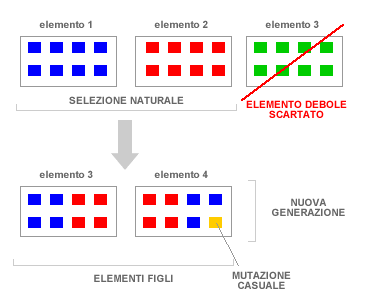
\includegraphics[width=0.5\textwidth]{img/algoritmo-genetico-schema.png}
    \caption{Schema Algortitmi Genetici. Immagine tratta da \cite{GA_Image}}
    \label{fig:Schema Algotmi Genetici}
\end{figure}

\subsection{Schema dell'Algoritmo Genetico}
Il ciclo evolutivo standard segue questi passaggi:
\begin{enumerate}
\item \textbf{Inizializzazione}: Genera una popolazione iniziale casuale
\item \textbf{Valutazione}: Calcola la fitness di ogni individuo
\item \textbf{Controllo terminazione}: Verifica i criteri di stop
\item \textbf{Selezione}: Sceglie i genitori per la riproduzione
\item \textbf{Crossover}: Applica ricombinazione con probabilità $p_c$
\item \textbf{Mutazione}: Applica mutazione con probabilità $p_m$
\item \textbf{Rimpiazzamento}: Determina la nuova popolazione
\item \textbf{Ritorna al passo 2}
\end{enumerate}

\subsection{Parametri e Tuning}
Il successo di un algoritmo genetico dipende criticamente dalla scelta dei parametri:
\begin{itemize}
\item \textbf{Dimensione popolazione}: Tipicamente 50-500 individui
\item \textbf{Probabilità di crossover}: Generalmente alta (0.6-0.9)
\item \textbf{Probabilità di mutazione}: Generalmente bassa (0.001-0.1)
\end{itemize}

\end{flushleft}

\section{Metodi di Crossover per Codifica Reale}
\begin{flushleft}
Quando si lavora con problemi di ottimizzazione continua, la codifica reale richiede operatori di crossover specificamente progettati per preservare e ricombinare efficacemente l'informazione numerica. I metodi principali si distinguono per le loro proprietà matematiche e il comportamento esplorativo.


\subsection{Crossover Aritmetico}
Il crossover aritmetico genera la prole come combinazione lineare dei genitori:
\[
\begin{aligned}
\text{figlio}_1 &= \alpha \cdot \text{genitore}_1 + (1-\alpha) \cdot \text{genitore}_2 \\
\text{figlio}_2 &= (1-\alpha) \cdot \text{genitore}_1 + \alpha \cdot \text{genitore}_2
\end{aligned}
\]
dove $\alpha \in [0,1]$ è un parametro che controlla il peso della combinazione.

\textbf{Varianti principali:}
\begin{itemize}
\item \textbf{Uniforme}: $\alpha$ costante per tutti i geni
\item \textbf{Non-uniforme}: $\alpha$ varia per ogni gene
\item \textbf{Adattivo}: $\alpha$ cambia nel tempo o in base alla fitness
\end{itemize}

\textbf{Proprietà:} Garantisce che la prole rimanga nell'ipercubo definito dai genitori, assicurando exploiting delle regioni promettenti.

\subsection{Blend Crossover (BLX)}
Il Blend Crossover, proposto da Eshelman e Schaffer, estende l'intervallo di ricombinazione oltre i valori dei genitori. Per ogni gene $i$:
\[
\text{figlio}_i \sim U[x_{\min} - \alpha \cdot I, x_{\max} + \alpha \cdot I]
\]
dove:
\begin{itemize}
\item $x_{\min} = \min(\text{genitore}_{1,i}, \text{genitore}_{2,i})$
\item $x_{\max} = \max(\text{genitore}_{1,i}, \text{genitore}_{2,i})$
\item $I = x_{\max} - x_{\min}$
\item $\alpha$ controlla l'estensione dell'intervallo (tipicamente 0.5)
\end{itemize}

\textbf{Caratteristiche:}
\begin{itemize}
\item Bilancia exploration ed exploitation
\item Mantiene diversità nella popolazione
\item Può generare valori esterni all'intervallo parentale
\end{itemize}

\subsection{Simulated Binary Crossover (SBX)}
Il Simulated Binary Crossover, sviluppato da Deb e Agrawal, simula il comportamento del crossover a punto singolo per variabili continue. La distribuzione di probabilità della prole è definita da:
\[
P(x) = \frac{1}{2}(\eta + 1)(1 - |x - 0.5|)^\eta
\]
dove $\eta$ è l'indice di distribuzione che controlla la forma della distribuzione.

\textbf{Procedura SBX:}
\begin{enumerate}
\item Genera un numero casuale $u \sim U[0,1]$
\item Calcola il fattore di espansione:
\[
\beta = \begin{cases}
(2u)^{1/(\eta+1)} & \text{se } u \leq 0.5 \\
(1/(2(1-u)))^{1/(\eta+1)} & \text{se } u > 0.5
\end{cases}
\]
\item Genera la prole:
\[
\begin{aligned}
\text{figlio}_1 &= 0.5[(1+\beta)\text{genitore}_1 + (1-\beta)\text{genitore}_2] \\
\text{figlio}_2 &= 0.5[(1-\beta)\text{genitore}_1 + (1+\beta)\text{genitore}_2]
\end{aligned}
\]
\end{enumerate}

\textbf{Vantaggi di SBX:}
\begin{itemize}
\item Controllo preciso della dispersione tramite $\eta$
\item Comportamento auto-adattivo rispetto alla distanza parentale
\item Ampiamente utilizzato in algoritmi evolutivi multi-obiettivo
\item Preserva la media dei genitori
\end{itemize}

\subsection{Confronto e Scelta del Metodo}
La scelta del metodo di crossover dipende dalle caratteristiche del problema:
\begin{itemize}
\item \textbf{Crossover aritmetico}: Ideale per exploitation locale e convergenza rapida
\item \textbf{BLX}: Bilanciato per problemi che richiedono exploration moderata
\item \textbf{SBX}: Preferito per ottimizzazione multi-obiettivo e controllo fine della dispersione
\end{itemize}

\end{flushleft}

\section{Rappresentazione di Reti Neurali attraverso i GA}
\begin{flushleft}
La rappresentazione di reti neurali attraverso algoritmi genetici costituisce un approccio alternativo ai metodi di addestramento tradizionali basati sul gradiente. Questo paradigma consente di formulare l'ottimizzazione dei parametri di rete come un problema di ricerca evolutiva, aprendo nuove possibilità per l'esplorazione dello spazio dei pesi e superando alcune limitazioni intrinseche dei metodi gradient-based.

\subsection{Codifica dei Parametri di Rete}
Per applicare gli algoritmi genetici all'addestramento di reti neurali, è necessario definire una rappresentazione appropriata che mappi la struttura della rete in un cromosoma evolutivo. L'approccio più diretto e comunemente utilizzato consiste nella \textbf{codifica diretta dei pesi}, dove ogni individuo della popolazione è rappresentato come un vettore di valori reali:

\[
\mathbf{x} = [w_1, w_2, \ldots, w_n, b_1, b_2, \ldots, b_m]
\]

dove $w_i$ rappresentano i pesi sinaptici e $b_j$ i bias della rete. Questa rappresentazione concatena linearmente tutti i parametri della rete in un singolo cromosoma, mantenendo un ordine consistente che preservi la topologia delle connessioni.

\textbf{Vantaggi della codifica diretta:}
\begin{itemize}
\item Semplicità implementativa e concettuale
\item Applicabilità a qualsiasi architettura di rete
\item Compatibilità diretta con operatori genetici standard per valori reali
\end{itemize}

\textbf{Limitazioni:}
\begin{itemize}
\item Scalabilità limitata per reti di grandi dimensioni
\item Perdita di informazione strutturale nel cromosoma
\item Crescita quadratica dello spazio di ricerca rispetto alla dimensione della rete
\end{itemize}


\subsection{Funzione di Fitness}
La definizione della funzione di fitness rappresenta un elemento cruciale che determina la direzione dell'evoluzione. A differenza dei metodi gradient-based, gli algoritmi genetici permettono di utilizzare qualsiasi metrica valutabile, anche non differenziabile.
\subsubsection{Metriche Basate sulla Loss}
Le funzioni di loss tradizionali possono essere utilizzate direttamente come funzione di fitness negli algoritmi genetici. Non esiste una rappresentazione obbligatoria per la trasformazione loss-fitness; l'aspetto cruciale consiste nel definire correttamente se l'obiettivo è la minimizzazione o la massimizzazione della metrica scelta.

Gli approcci principali includono:
\begin{itemize}
\item \textbf{Utilizzo diretto}: Configurare l'algoritmo genetico per minimizzare la loss
\item \textbf{Negazione}: Utilizzare $\text{fitness} = -\text{loss}$ per massimizzazione
\item \textbf{Trasformazioni}: Applicare funzioni come $\text{fitness} = \frac{1}{1 + \text{loss}}$ per mappare in valori positivi
\end{itemize}

Le loss più comuni includono:
\begin{itemize}
\item \textbf{Mean Squared Error (MSE)}: $\text{MSE} = \frac{1}{N}\sum_{i=1}^{N}(y_i - \hat{y}_i)^2$
\item \textbf{Cross-Entropy}: $\text{CE} = -\frac{1}{N}\sum_{i=1}^{N}\sum_{c=1}^{C}y_{i,c}\log(\hat{y}_{i,c})$
\end{itemize}

\subsubsection{Metriche Alternative Non Differenziabili}
Una caratteristica distintiva degli algoritmi genetici è la possibilità di ottimizzare direttamente metriche di performance che non sono differenziabili, aprendo nuovi scenari di ottimizzazione:

\textbf{Accuracy:} La percentuale di predizioni corrette può essere utilizzata direttamente:
\[
\text{Accuracy} = \frac{1}{N}\sum_{i=1}^{N}\mathbb{I}[\arg\max(\hat{y}_i) = \arg\max(y_i)]
\]

\textbf{F1-Score:} Particolarmente utile per dataset sbilanciati:
\[
\text{F1} = \frac{2 \cdot \text{Precision} \cdot \text{Recall}}{\text{Precision} + \text{Recall}}
\]

\textbf{Metriche composite:} È possibile combinare multiple obiettivi:
\[
\text{fitness} = \alpha \cdot \text{Accuracy} + \beta \cdot \text{Complessità}^{-1} + \gamma \cdot \text{Robustezza}
\]


\subsection{Confronto con Metodi Gradient-Based}
L'utilizzo di algoritmi genetici per l'addestramento di reti neurali presenta caratteristiche distintive rispetto ai metodi tradizionali:

\textbf{Vantaggi degli algoritmi genetici:}
\begin{itemize}
\item \textbf{Robustezza ai minimi locali}: L'esplorazione population-based riduce il rischio di convergenza prematura
\item \textbf{Flessibilità nella funzione obiettivo}: Possibilità di ottimizzare metriche non differenziabili
\item \textbf{Parallelizzazione naturale}: La valutazione degli individui è intrinsecamente parallelizzabile
\item \textbf{Resistenza al rumore}: Meno sensibili a valutazioni fitness rumorose
\end{itemize}

\textbf{Limitazioni rispetto ai metodi gradient-based:}
\begin{itemize}
\item \textbf{Efficienza computazionale}: Richiedono tipicamente più valutazioni della funzione obiettivo
\item \textbf{Scalabilità}: Problematici per reti con milioni di parametri
\item \textbf{Convergenza}: Generalmente più lenti nella fase di fine-tuning locale
\end{itemize}

Questa dualità di approcci evidenzia come gli algoritmi genetici possano essere particolarmente vantaggiosi in scenari specifici, quali l'ottimizzazione di architetture di rete, l'addestramento in ambienti multi-obiettivo, o quando la funzione di loss presenta caratteristiche non favorevoli ai metodi basati sul gradiente.

\end{flushleft}

\section{Conclusioni}
\begin{flushleft}
In questo capitolo sono stati presentati gli algoritmi evolutivi in generale e gli algoritmi genetici nello specifico. Sono stati analizzati i passaggi e le componenti principali che li caratterizzano, dedicando particolare attenzione ai diversi operatori genetici e focalizzandosi approfonditamente sui vari metodi di crossover, che rappresentano uno degli elementi fondamentali dei GA.

È stata inoltre esaminata la modalità di codifica e addestramento delle reti neurali attraverso l'utilizzo degli algoritmi genetici, evidenziando come questo approccio alternativo possa superare alcune limitazioni dei metodi tradizionali basati sul gradiente. Questa introduzione teorica costituisce la base necessaria per comprendere pienamente i capitoli successivi, dove verrà definita l'architettura specifica della rete neurale utilizzata, la sua rappresentazione attraverso GA, i metodi di crossover e mutazione implementati, nonché ulteriori tecniche di ottimizzazione applicate.


\end{flushleft}